\chapter*{Appendix} \label{chp:appendix}
\section{Proofs}
\begin{proof} \label{proof:insertionSearch}
Given a set of cognitive operations $M$, an external activation function $f()$, and an initially valid SCP $f(\pi)$, $\pi=\{s_i \longmapsto A_0 \longmapsto ... \longmapsto A_n\}$, $A_i \in M$, inserting multiple operations into $\pi$ to create cognitive sequence $\pi'$ may result in a valid SCP $f(\pi')$, when inserting only one operation would result in an invalid SCP.

\begin{itemize}
\item Assume hybrid validity (Section~@TODOsection).
\item Let $f(\pi)=\{True if V is defined\}$, $\gamma = True$.
\item Let $A_x$ be a cognitive operation which transforms an input state point of structure $\{KB, V\}$, where $KB$ contains a set of logical formula of the form $head \leftarrow body$ and every rule in $V$ is of the form $variable \leftarrow value$, where $variable$ is an atom and  $value=\top$ into an output state point of structure $\{KB'\}$, $KB'=(KB \cup V)$.
\item Let $A_y$ be cognitive operation which transforms an input state point of structure $KB'$ into an output state point of structure $\{KB, V\}$ where $V$ contains every rule of the form $head \leftarrow body$, where $head$ is an atom and $body=\top$ and $KB= KB' \setminus V$.
\end{itemize}
\item if $f(\pi)$, $pi=(s_i)$ is a valid SCP, then $f(\pi')$, $\pi'=(s_i\longmapsto A_x)$ is an invalid SCP and $f(\pi'')$, $\pi''=(\pi'\longmapsto A_y)$ is valid.
\end{proof}

\begin{proof} \label{proof:infiniteSCPLength}
If there exists an SCP which meets goal condition $\gamma$ of length $n$, then there exists an SCP that meets goal condition $\gamma$ of length $n+k$ where $k$ is any natural number.
\begin{itemize}

\item Proof~\ref{proof:infiniteSCPs} states that if $f(x \longmapsto A)\models \gamma$ then $f(x \longmapsto T_i \longmapsto V_i)\models \gamma$ for all $(T_i \in T, P_i \in P) \in W$.
\item Let $X$ be a partial SCP of the form $X=T_0 \longmapsto V_0 \longmapsto ... \longmapsto T_N \longmapsto V_{N}$ where $(V_i, T_i) \in W$
\item For odd lengths:
\begin{itemize}
\item  It follows that if $f(x \longmapsto A)\models \gamma$ then $f(x \longmapsto A \longmapsto \textrm{exp}(X))\models \gamma$, where $\textrm{exp}$ denotes the substitution of $X$ for its constituent parts.
\item Because $X$ always contains an even number of cognitive operations, then the length of the resulting SCP must be $n' = 1+v$ where $v$ is any even number.
\end{itemize}
\item For even lengths:
\begin{itemize}
\item Notice that $f(x \longmapsto A \longmapsto \textrm{exp}(X) \longmapsto X) \models \gamma$.
\item A appending $\longmapsto X$ to adds one to the length of any SCP.
\item Because we have shown that a suitable SCP of any odd length exists $n'>=n$, it follows that a suitable SCP of any even length $n'>n$ exists.
\end{itemize}
\end{itemize}

\end{proof}

\begin{lemma} \label{lem:uniredundant}
Given a cognitive operation sequence $A \in \Omega^*$, and external function $f()$, $A$ is redundant redundant iff one of the following holds:
\begin{itemize}
\item $(x \longmapsto B \longmapsto C) \models x'$ and $(x \longmapsto A) \models x'$ for every viable epistemic state $x$, $B \in \Omega^*$, $C \in \Omega^*$. 
\item $x \longmapsto A \models x$ for every viable epistemic state $x$.
\item $f(x \longmapsto B)=c$ for all $B \in \Omega^*$, where $c$ is a constant external decision.
\end{itemize}
\end{lemma}

\begin{lemma} \label{lem:taskredundant}
Given a limited set of cognitive operations $M=\{A_0, ..., A_n\}, A_x \in \Omega^*$, and external function $f()$, $A \in M^*$ is task redundant iff one of the following holds:
\begin{itemize}
\item $(x \longmapsto B \longmapsto C) \models x'$ and $(x \longmapsto A) \models x'$ for every viable epistemic state $x$, $B \in M^*$, $C \in M^*$. 
\item $x \longmapsto A \models x$ for every viable epistemic state $x$.
\item $f(x \longmapsto B)=c$ for all $B \in M^*$, where $c$ is a constant external decision.
\item There exists no epistemic state $x$ and sequences $B, C \in M^*$ such that $f(x \longmapsto B \longmapsto A \longmapsto C)$ is a valid SCP.
\end{itemize}
\end{lemma}

\begin{proof} \label{proof:aggregateExpressiveness}
Given a cognitive task $\Pi=(x,f(), M, \gamma)$ in which $M=\{A_0,...,A_n\}$ and a second cognitive planing task $\Pi'=(x,f(),M')$ in which $M'= M \smallsetminus \{A_k,...,A_m\} \cup A'$, where $A'=(A_k \longmapsto... \longmapsto A_m)$ is a cognitive sequence containing some ordering of the other operations in $(\Pi \smallsetminus \Pi')$, $\Pi'$ is as expressive or less expressive than $\Pi$.

\item No more expressive:
\begin{itemize}
\item If $\pi' = (x\longmapsto A_p \longmapsto ... \longmapsto A' \longmapsto ... \longmapsto A_q)$ and $f(\pi)$ is a solution to $\Pi'$.
\item Let $\pi'' = (x\longmapsto A_p \longmapsto ... \longmapsto [A'] \longmapsto ... \longmapsto A_q)$.
\item Then $f(\pi'')$ is a solution to $\Pi'$ (Lemma~\ref{lemma:substitutionValid}).
\item $f(\pi'')$ is a valid solution to $\Pi$ because $\pi''$ uses only cognitive operations which occur in $\Pi$, $x$ is the initial epistemic state, and $f(\pi'') \models \gamma$. 
\end{itemize}

\item Less Expressive: Proof by counterexample
\begin{itemize}
\item If we assume that $\Pi'$ is strictly as expressive or more expressive than $\Pi$, then there exist no cases in which $\Pi'$ is less expressive.
\item Let $\gamma = \emptyset$, and $f(x)=True$ for all inputs (i.e. is trivially satisfied).
\item Let $x=\{\}$, $M=\{A_0,A_1\}$, $M'=\{A'\}$, $A'=\{A_0\longmapsto A_1\}$.
\item Then solutions of $\Pi$ are $f(x)$, $f(x \longmapsto A_0)$, $f(x \longmapsto A_1)$, $f(x \longmapsto A_0\longmapsto A_1)$ and $f(x \longmapsto A_1\longmapsto A_0)$.
\item Solutions of $\Pi'$ are $f(x), f(x \longmapsto A')$.
\item Thus, $\Pi'$ has fewer solutions that $\Pi$. A contradiction.
\end{itemize}
\end{proof}

\begin{proof} \label{proof:aggregateValid}
Given an SCP $\pi= f(x \longmapsto A_0 \longmapsto ... \longmapsto A_n)$, where $f(x)$ is an external evaluation function, $x$ is a state point, and $A_i \in \Omega$, any subsequence $A'=(A_k \longmapsto ... \longmapsto A_{k+l})$, $(k+l)<n$ of the cognitive operations in $\pi$ is a valid cognitive operation.
\begin{itemize}
\item Given that $\pi$ is a valid SCP, $x \longmapsto A_0$ must, by the definitions discussed in Section~@TODOref result in a valid state point.
\item It follows that $A'$ takes a valid state point as input, because $A_k$ took a valid state point as input.
\item It follows that $A'$ produces a valid state point as output, because $A_{k+1}$ produced a valid state point as output.
\item Therefore, $A'$ is a valid cognitive operation, by the definition in Section~@TODOref.
\end{itemize}
\end{proof}

\begin{lemma} \label{lemma:substitutionValid}
Let $\pi=(x\longmapsto A_0, ..., A', ..., longmapsto A_n)$ be a sequence of cognitive operations drawn from some cognitive task $\Pi=(x, \gamma, f(x), M)$ . And let $\pi'=(x\longmapsto [A_0], ..., A', ..., longmapsto A_n)$ where $[A]$ is the substitution of the aggregate operation $A'$ for $(A'[0]\longmapsto ... \longmapsto A'[t])$ . Then $f(\pi)=f(\pi')$.
\end{lemma}

\begin{proof} \label{proof:infiniteSCPs}
There are an infinite number of possible, valid SCPs, that can meet any goal condition $\gamma$ from input $x$ provided that at least one SCP exists that can reach goal condition $\gamma$ from input $x$.
\begin{enumerate}
\item There exist infinitely many cognitive operations $T \in \Omega$ which add a new variable from the set of all possible variable names $p \in P$.
\item There exist infinitely many cognitive operations $V \in \Omega$ which remove a variable from the set of all possible variable names  $p \in P$.
\item It follows that there exist infinitely many pairs $(T_i \in T, P_i \in P) \in W$ where $T_i$ adds a variable $p \in P$ to the resulting state point, and $V_i$ removes that variable from the resulting statepoint.
\item Then $f(x \longmapsto A) = f(x \longmapsto T_i \longmapsto V_i)$
\item Thus it follows that if $f(x \longmapsto A)\models \gamma$ then $f(x \longmapsto T_i \longmapsto V_i)\models \gamma$ for all $(T_i \in T, P_i \in P) \in W$.
\end{enumerate}
\end{proof}

\section{Output}


\section{Code Snippets}
\subsection{Program Flow}
\begin{figure}
\centering 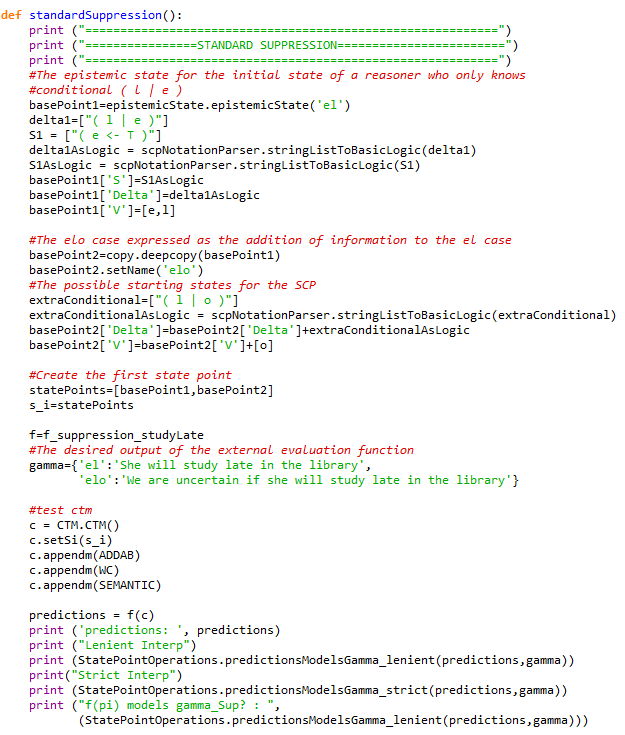
\includegraphics[width=\linewidth]{suppression_python}
\caption{Code snippet showing how the Suppression Task is modelled in the SCP Framework}.
\label{fig:suppression_python}
\end{figure}

